%% bare_conf.tex
%% V1.3
%% 2007/01/11
%% by Michael Shell
%% See:
%% http://www.michaelshell.org/
%% for current contact information.
%%
%% This is a skeleton file demonstrating the use of IEEEtran.cls
%% (requires IEEEtran.cls version 1.7 or later) with an IEEE conference paper.
%%
%% Support sites:
%% http://www.michaelshell.org/tex/ieeetran/
%% http://www.ctan.org/tex-archive/macros/latex/contrib/IEEEtran/
%% and
%% http://www.ieee.org/

%%*************************************************************************
%% Legal Notice:
%% This code is offered as-is without any warranty either expressed or
%% implied; without even the implied warranty of MERCHANTABILITY or
%% FITNESS FOR A PARTICULAR PURPOSE! 
%% User assumes all risk.
%% In no event shall IEEE or any contributor to this code be liable for
%% any damages or losses, including, but not limited to, incidental,
%% consequential, or any other damages, resulting from the use or misuse
%% of any information contained here.
%%
%% All comments are the opinions of their respective authors and are not
%% necessarily endorsed by the IEEE.
%%
%% This work is distributed under the LaTeX Project Public License (LPPL)
%% ( http://www.latex-project.org/ ) version 1.3, and may be freely used,
%% distributed and modified. A copy of the LPPL, version 1.3, is included
%% in the base LaTeX documentation of all distributions of LaTeX released
%% 2003/12/01 or later.
%% Retain all contribution notices and credits.
%% ** Modified files should be clearly indicated as such, including  **
%% ** renaming them and changing author support contact information. **
%%
%% File list of work: IEEEtran.cls, IEEEtran_HOWTO.pdf, bare_adv.tex,
%%                    bare_conf.tex, bare_jrnl.tex, bare_jrnl_compsoc.tex
%%*************************************************************************

% *** Authors should verify (and, if needed, correct) their LaTeX system  ***
% *** with the testflow diagnostic prior to trusting their LaTeX platform ***
% *** with production work. IEEE's font choices can trigger bugs that do  ***
% *** not appear when using other class files.                            ***
% The testflow support page is at:
% http://www.michaelshell.org/tex/testflow/



% Note that the a4paper option is mainly intended so that authors in
% countries using A4 can easily print to A4 and see how their papers will
% look in print - the typesetting of the document will not typically be
% affected with changes in paper size (but the bottom and side margins will).
% Use the testflow package mentioned above to verify correct handling of
% both paper sizes by the user's LaTeX system.
%
% Also note that the "draftcls" or "draftclsnofoot", not "draft", option
% should be used if it is desired that the figures are to be displayed in
% draft mode.
%
\documentclass[conference]{IEEEtran}
% Add the compsoc option for Computer Society conferences.
%
% If IEEEtran.cls has not been installed into the LaTeX system files,
% manually specify the path to it like:
% \documentclass[conference]{../sty/IEEEtran}





% Some very useful LaTeX packages include:
% (uncomment the ones you want to load)


% *** MISC UTILITY PACKAGES ***
%
%\usepackage{ifpdf}
% Heiko Oberdiek's ifpdf.sty is very useful if you need conditional
% compilation based on whether the output is pdf or dvi.
% usage:
% \ifpdf
%   % pdf code
% \else
%   % dvi code
% \fi
% The latest version of ifpdf.sty can be obtained from:
% http://www.ctan.org/tex-archive/macros/latex/contrib/oberdiek/
% Also, note that IEEEtran.cls V1.7 and later provides a builtin
% \ifCLASSINFOpdf conditional that works the same way.
% When switching from latex to pdflatex and vice-versa, the compiler may
% have to be run twice to clear warning/error messages.

% *** CITATION PACKAGES ***
%
%\usepackage{cite}
\usepackage{cite}
% cite.sty was written by Donald Arseneau
% V1.6 and later of IEEEtran pre-defines the format of the cite.sty package
% \cite{} output to follow that of IEEE. Loading the cite package will
% result in citation numbers being automatically sorted and properly
% "compressed/ranged". e.g., [1], [9], [2], [7], [5], [6] without using
% cite.sty will become [1], [2], [5]--[7], [9] using cite.sty. cite.sty's
% \cite will automatically add leading space, if needed. Use cite.sty's
% noadjust option (cite.sty V3.8 and later) if you want to turn this off.
% cite.sty is already installed on most LaTeX systems. Be sure and use
% version 4.0 (2003-05-27) and later if using hyperref.sty. cite.sty does
% not currently provide for hyperlinked citations.
% The latest version can be obtained at:
% http://www.ctan.org/tex-archive/macros/latex/contrib/cite/
% The documentation is contained in the cite.sty file itself.






% *** GRAPHICS RELATED PACKAGES ***
%
\ifCLASSINFOpdf
  % \usepackage[pdftex]{graphicx}
  % declare the path(s) where your graphic files are
  % \graphicspath{{../pdf/}{../jpeg/}}
  % and their extensions so you won't have to specify these with
  % every instance of \includegraphics
  % \DeclareGraphicsExtensions{.pdf,.jpeg,.png}
\else
  % or other class option (dvipsone, dvipdf, if not using dvips). graphicx
  % will default to the driver specified in the system graphics.cfg if no
  % driver is specified.
   \usepackage[dvips]{graphicx}
  % declare the path(s) where your graphic files are
   \graphicspath{{../figures/}}
  % and their extensions so you won't have to specify these with
  % every instance of \includegraphics
   \DeclareGraphicsExtensions{.eps}
\fi
% graphicx was written by David Carlisle and Sebastian Rahtz. It is
% required if you want graphics, photos, etc. graphicx.sty is already
% installed on most LaTeX systems. The latest version and documentation can
% be obtained at: 
% http://www.ctan.org/tex-archive/macros/latex/required/graphics/
% Another good source of documentation is "Using Imported Graphics in
% LaTeX2e" by Keith Reckdahl which can be found as epslatex.ps or
% epslatex.pdf at: http://www.ctan.org/tex-archive/info/
%
% latex, and pdflatex in dvi mode, support graphics in encapsulated
% postscript (.eps) format. pdflatex in pdf mode supports graphics
% in .pdf, .jpeg, .png and .mps (metapost) formats. Users should ensure
% that all non-photo figures use a vector format (.eps, .pdf, .mps) and
% not a bitmapped formats (.jpeg, .png). IEEE frowns on bitmapped formats
% which can result in "jaggedy"/blurry rendering of lines and letters as
% well as large increases in file sizes.
%
% You can find documentation about the pdfTeX application at:
% http://www.tug.org/applications/pdftex





% *** MATH PACKAGES ***
%
\usepackage[cmex10]{amsmath}
% A popular package from the American Mathematical Society that provides
% many useful and powerful commands for dealing with mathematics. If using
% it, be sure to load this package with the cmex10 option to ensure that
% only type 1 fonts will utilized at all point sizes. Without this option,
% it is possible that some math symbols, particularly those within
% footnotes, will be rendered in bitmap form which will result in a
% document that can not be IEEE Xplore compliant!
%
% Also, note that the amsmath package sets \interdisplaylinepenalty to 10000
% thus preventing page breaks from occurring within multiline equations. Use:
%\interdisplaylinepenalty=2500
% after loading amsmath to restore such page breaks as IEEEtran.cls normally
% does. amsmath.sty is already installed on most LaTeX systems. The latest
% version and documentation can be obtained at:
% http://www.ctan.org/tex-archive/macros/latex/required/amslatex/math/





% *** SPECIALIZED LIST PACKAGES ***
%
%\usepackage{algorithmic}
% algorithmic.sty was written by Peter Williams and Rogerio Brito.
% This package provides an algorithmic environment fo describing algorithms.
% You can use the algorithmic environment in-text or within a figure
% environment to provide for a floating algorithm. Do NOT use the algorithm
% floating environment provided by algorithm.sty (by the same authors) or
% algorithm2e.sty (by Christophe Fiorio) as IEEE does not use dedicated
% algorithm float types and packages that provide these will not provide
% correct IEEE style captions. The latest version and documentation of
% algorithmic.sty can be obtained at:
% http://www.ctan.org/tex-archive/macros/latex/contrib/algorithms/
% There is also a support site at:
% http://algorithms.berlios.de/index.html
% Also of interest may be the (relatively newer and more customizable)
% algorithmicx.sty package by Szasz Janos:
% http://www.ctan.org/tex-archive/macros/latex/contrib/algorithmicx/




% *** ALIGNMENT PACKAGES ***
%
%\usepackage{array}
% Frank Mittelbach's and David Carlisle's array.sty patches and improves
% the standard LaTeX2e array and tabular environments to provide better
% appearance and additional user controls. As the default LaTeX2e table
% generation code is lacking to the point of almost being broken with
% respect to the quality of the end results, all users are strongly
% advised to use an enhanced (at the very least that provided by array.sty)
% set of table tools. array.sty is already installed on most systems. The
% latest version and documentation can be obtained at:
% http://www.ctan.org/tex-archive/macros/latex/required/tools/


%\usepackage{mdwmath}
%\usepackage{mdwtab}
% Also highly recommended is Mark Wooding's extremely powerful MDW tools,
% especially mdwmath.sty and mdwtab.sty which are used to format equations
% and tables, respectively. The MDWtools set is already installed on most
% LaTeX systems. The lastest version and documentation is available at:
% http://www.ctan.org/tex-archive/macros/latex/contrib/mdwtools/


% IEEEtran contains the IEEEeqnarray family of commands that can be used to
% generate multiline equations as well as matrices, tables, etc., of high
% quality.


%\usepackage{eqparbox}
% Also of notable interest is Scott Pakin's eqparbox package for creating
% (automatically sized) equal width boxes - aka "natural width parboxes".
% Available at:
% http://www.ctan.org/tex-archive/macros/latex/contrib/eqparbox/

\usepackage{array}
\usepackage{tabularx,ragged2e,booktabs}

% *** SUBFIGURE PACKAGES ***
%\usepackage[font={small}]{caption, subfig}
\usepackage[font={footnotesize}]{caption, subfig}
%\usepackage[tight,footnotesize]{subfigure}
% subfigure.sty was written by Steven Douglas Cochran. This package makes it
% easy to put subfigures in your figures. e.g., "Figure 1a and 1b". For IEEE
% work, it is a good idea to load it with the tight package option to reduce
% the amount of white space around the subfigures. subfigure.sty is already
% installed on most LaTeX systems. The latest version and documentation can
% be obtained at:
% http://www.ctan.org/tex-archive/obsolete/macros/latex/contrib/subfigure/
% subfigure.sty has been superceeded by subfig.sty.



%\usepackage{caption}
%\usepackage[font=footnotesize]{subfig}
% subfig.sty, also written by Steven Douglas Cochran, is the modern
% replacement for subfigure.sty. However, subfig.sty requires and
% automatically loads Axel Sommerfeldt's caption.sty which will override
% IEEEtran.cls handling of captions and this will result in nonIEEE style
% figure/table captions. To prevent this problem, be sure and preload
% caption.sty with its "caption=false" package option. This is will preserve
% IEEEtran.cls handing of captions. Version 1.3 (2005/06/28) and later 
% (recommended due to many improvements over 1.2) of subfig.sty supports
% the caption=false option directly:
%\usepackage[caption=false,font=footnotesize]{subfig}
%
% The latest version and documentation can be obtained at:
% http://www.ctan.org/tex-archive/macros/latex/contrib/subfig/
% The latest version and documentation of caption.sty can be obtained at:
% http://www.ctan.org/tex-archive/macros/latex/contrib/caption/

% *** FLOAT PACKAGES ***
%
%\usepackage{fixltx2e}
% fixltx2e, the successor to the earlier fix2col.sty, was written by
% Frank Mittelbach and David Carlisle. This package corrects a few problems
% in the LaTeX2e kernel, the most notable of which is that in current
% LaTeX2e releases, the ordering of single and double column floats is not
% guaranteed to be preserved. Thus, an unpatched LaTeX2e can allow a
% single column figure to be placed prior to an earlier double column
% figure. The latest version and documentation can be found at:
% http://www.ctan.org/tex-archive/macros/latex/base/



\usepackage{stfloats}
% stfloats.sty was written by Sigitas Tolusis. This package gives LaTeX2e
% the ability to do double column floats at the bottom of the page as well
% as the top. (e.g., "\begin{figure*}[!b]" is not normally possible in
% LaTeX2e). It also provides a command:
%\fnbelowfloat
% to enable the placement of footnotes below bottom floats (the standard
% LaTeX2e kernel puts them above bottom floats). This is an invasive package
% which rewrites many portions of the LaTeX2e float routines. It may not work
% with other packages that modify the LaTeX2e float routines. The latest
% version and documentation can be obtained at:
% http://www.ctan.org/tex-archive/macros/latex/contrib/sttools/
% Documentation is contained in the stfloats.sty comments as well as in the
% presfull.pdf file. Do not use the stfloats baselinefloat ability as IEEE
% does not allow \baselineskip to stretch. Authors submitting work to the
% IEEE should note that IEEE rarely uses double column equations and
% that authors should try to avoid such use. Do not be tempted to use the
% cuted.sty or midfloat.sty packages (also by Sigitas Tolusis) as IEEE does
% not format its papers in such ways.

% *** PDF, URL AND HYPERLINK PACKAGES ***
%
%\usepackage{url}
% url.sty was written by Donald Arseneau. It provides better support for
% handling and breaking URLs. url.sty is already installed on most LaTeX
% systems. The latest version can be obtained at:
% http://www.ctan.org/tex-archive/macros/latex/contrib/misc/
% Read the url.sty source comments for usage information. Basically,
% \url{my_url_here}.
%% Package to linebreak URLs in a sane manner.
\usepackage{url}
%% Define a new 'smallurl' style for the package that will use a smaller font.
\makeatletter
\def\url@smallurlstyle{%
  \@ifundefined{selectfont}{\def\UrlFont{\sf}}{\def\UrlFont{\small\ttfamily}}}
\makeatother
%% Now actually use the newly defined style.
\urlstyle{smallurl}
%% Define 'tinyurl' style for even smaller URLs (such as in tables)
\makeatletter
\def\url@tinyurlstyle{%
  \@ifundefined{selectfont}{\def\UrlFont{\sf}}{\def\UrlFont{\scriptsize\ttfamily}}}
\makeatother
\renewcommand{\UrlFont}{\scriptsize}
%
%% Make URLs clickable
\usepackage[colorlinks, bookmarks=false]{hyperref}
%\usepackage{hyperref}
\usepackage{breakurl}
\hypersetup{
    %linktoc=all,     %set to all if you want both sections and subsections linked
    %linkcolor=blue,  %choose some color if you want links to stand out
    colorlinks=false, %set true if you want colored links
    citecolor=black,
    filecolor=black,
    linkcolor=black,
    urlcolor=black
}

%% Squeezing the paper a bit
%
% reduce the white space around figures and tables centrally
%\newcommand{\myfigureshrinker}{\vspace{0.03cm}}
%\newcommand{\myfigureshrinkerless}{\vspace{-0.03cm}}
%
% slightly reduce the space between the lines. To do that you can insert a line like
\def\baselinestretch{1}
%
%
%The fonts of the caption can be centrally changed using the caption package:
%\usepackage[font={small}]{caption, subfig}
%
% A little bit of space can be gained by abbreviating references
\renewcommand{\figurename}{Fig.}
\renewcommand{\tablename}{Tab.}
%
% it is possible to change the spacing in and around floats using these lengths
\setlength{\abovecaptionskip}{1ex}
\setlength{\belowcaptionskip}{2.5ex}
\setlength{\floatsep}{1ex}
\setlength{\textfloatsep}{1ex}
%
%
%make sure the citations in the text take as little space as possible:
%\usepackage[sort&compress]{natbib}    
%Make the font of the references smaller
\newcommand{\bibfont}{\small}
%Reduce the spaces between the individual references
%\setlength{\bibsep}{0ex}
%
% Changing math formatting
%
\DeclareMathSizes{10}{9}{6}{5}
\abovedisplayskip.50ex
\belowdisplayskip.50ex
\abovedisplayshortskip.50ex
\belowdisplayshortskip.50ex

%
%\addtolength{\topmargin}{-9mm}
%\addtolength{\topskip}{-6mm}
\addtolength{\textfloatsep}{-4mm}
\addtolength{\dbltextfloatsep}{-4mm}

%\renewcommand\floatpagefraction{.9}
%\renewcommand\topfraction{.9}
%\renewcommand\bottomfraction{.9}
%\renewcommand\textfraction{.1}   
%\setcounter{totalnumber}{50}
%\setcounter{topnumber}{50}
%\setcounter{bottomnumber}{50}
\usepackage{microtype}

% *** Do not adjust lengths that control margins, column widths, etc. ***
% *** Do not use packages that alter fonts (such as pslatex).         ***
% There should be no need to do such things with IEEEtran.cls V1.6 and later.
% (Unless specifically asked to do so by the journal or conference you plan
% to submit to, of course. )

% correct bad hyphenation here
\hyphenation{op-tical net-works semi-conduc-tor}


\begin{document}
%
% paper title
% can use linebreaks \\ within to get better formatting as desired
\title{SAX-VSM: Interpretable Time Series Classification\\ Using SAX and Vector Space Model}

% author names and affiliations
% use a multiple column layout for up to three different
% affiliations
 \author{\IEEEauthorblockN{Pavel Senin}
 \IEEEauthorblockA{Information and Computer Sciences Department,\\
 University of Hawaii at Manoa, Honolulu, HI, 96822\\
 senin@hawaii.edu}
 \and
 \IEEEauthorblockN{Sergey Malinchik}
 \IEEEauthorblockA{Lockheed Martin Advanced Technology Laboratories,\\
 3 Executive Campus, Suite 600, Cherry Hill, NJ, 08002\\
 sergey.b.malinchik@lmco.com}}
\maketitle
%\bigskip

\begin{abstract}
%\boldmath
In this paper, we propose a novel method for characteristic patterns discovery in 
time series. This method, called SAX-VSM, is based on two existing techniques - 
Symbolic Aggregate approXimation and Vector Space Model. SAX-VSM is capable 
to automatically discover and rank time series patterns by their 
“importance” to the class, which not only creates well-performing classifiers,
but also provides an interpretable class generalization. 
The accuracy of the method, as shown through experimental evaluation, is at the 
level of the current state of the art. 
While being relatively computationally expensive within a learning phase, 
our method provides fast, precise, and interpretable classification.
\end{abstract}
% IEEEtran.cls defaults to using nonbold math in the Abstract.
% This preserves the distinction between vectors and scalars. However,
% if the conference you are submitting to favors bold math in the abstract,
% then you can use LaTeX's standard command \boldmath at the very start
% of the abstract to achieve this. Many IEEE journals/conferences frown on
% math in the abstract anyway.

% no keywords

% For peer review papers, you can put extra information on the cover
% page as needed:
 %\ifCLASSOPTIONpeerreview
 %\begin{center} \bfseries EDICS Category: 3-BBND \end{center}
 %\fi
%
% For peerreview papers, this IEEEtran command inserts a page break and
% creates the second title. It will be ignored for other modes.
%\IEEEpeerreviewmaketitle

%\enlargethispage{0.5cm}
\section{Introduction}
Time series classification is an increasingly popular area of research providing 
solutions to the wide range of fields including data mining, 
image and motion recognition, environmental sciences, health care, and chemometrics. 
Within last decades, many time series representations, similarity measures, 
and classification algorithms were proposed following the rapid
progress in data collection and storage technologies \cite{review}. 
Nevertheless, to date, the best overall performing classifier in the field is
a nearest-neighbor algorithm (1NN), that can be easily tuned for a 
particular problem by the choice of a distance measure, 
an approximation technique, or smoothing \cite{review}
%\cite{comparison}. 
%As pointed out by dozens of papers, 
1NN classifier is simple, accurate and robust, depends on a very few parameters 
and requires no training \cite{review, benchmark, classifiers}.
%\cite{review, benchmark, comparison, classifiers}.
However, while possessing these qualities, 1NN technique has a number of 
significant disadvantages, where the major shortcoming is that it does not 
offer any insight into the classification results.
Another limitation is its need for a significantly large training set 
representing a within-class variance in order to achieve a good accuracy. 
Finally, while having trivial initialization, 1NN classification is computationally expensive. 
Thus, the demand for an efficient and interpretable classification technique 
capable of processing of large data collections remains.

In this work, we propose an alternative to 1NN algorithm that addresses 
aforementioned limitations and provides a superior interpretability, 
learns efficiently from a small training set, and has a low classification 
computational complexity.

The paper is structured as follows: 
Section \ref{prior} discusses relevant work, Section \ref{background} provides 
background for a proposed algorithm, in Section \ref{sax-vsm} we describe our algorithm, 
and in Section \ref{results} we evaluate its performance. 
We conclude and discuss future work in Section \ref{conclusion}.

\vspace{-0.2cm}
\section{Prior and related work} \label{prior}
\vspace{-0.1cm}
Almost all of the existing techniques for time series classification can be divided 
in two major categories \cite{comparison}. 
The first category includes techniques based on shape-based similarity metrics 
where distance is measured directly between time series points. 
Classical examples from this category is 1NN classifier 
built upon Euclidean distance \cite{1NN} or DTW \cite{DTW}. 
The second category consists of classification techniques based on 
structural similarity metrics which employ a high-level representations 
of time series based on their global or local features. 
Examples from this category include a classifier based on 
DFT \cite{DFT} and a classifier based on Bag-Of-Patterns representation 
\cite{bag_patterns}. 
The development of these distinct categories can be explained by 
the difference in their performance: 
while shape-based similarity methods are virtually unbeatable on short 
pre-processed time series \cite{benchmark}, 
they usually fail on long and noisy data, where structure-based solutions 
demonstrate a superior performance \cite{bag_patterns}. 
%In addition, structure-based methods require less storage space and, usually, 
%have a faster classification time, thus, they often implemented in industrial settings. 

%Additionally, in the context of our work, it is worth to note, that classification 
%techniques from both categories can be also attributed as exact or approximate.
%While former are based on exact metrics, and typically are brute force 
%algorithms which guarantee results through an exhaustive search, 
%the latter are usually built upon an approximate representation of 
%time series, or upon an approximate similarity metric, and do not guarantee 
%global correctness. Nevertheless, while allowing a higher error rate,
%approximate techniques effectively reduce the search space, thus dealing with 
%large unprocessed data much more efficiently \cite{paa, sax, streaming_sax}.

%
%Further, similarity search techniques can be further categorized as exact 
%or approximate, where fast but approximate retrieval is often preferred over an 
%exact but slower one with the current growth of the data volumes, .
%
%As per current state of the art, it is worth noting, that despite to recent development,
%to date,
%the best algorithm in overall performance is the simple nearest neighbor classifier, that is
%accurate and robust \cite{review, benchmark, comparison, classifiers}. Moreover, it depends on a
%very few parameters. Nevertheless, while possessing all these qualities, 1NN technique has a n
%umber of disadvantages, where the major is that it does not offer any insight into the data, 
%while the next is the need for a significantly large training set.

%Recently, two relevant to our work techniques, were proposed. 
As possible alternatives to these two categories, two relevant to our work techniques, 
were recently proposed. 
The first is Time Series Shapelet technique introduced in \cite{shapelet} which
is featuring a superior interpretability and a compactness of delivered solution. 
A Shapelet is a short time series ``snippet'' that is a representative of class
membership and is used for a decision tree construction facilitating class 
identification and interpretability.
In order to find a branching shapelet, the algorithm exhaustively searches for a best 
discriminatory shapelet on data split via an information gain measure. 
The algorithm's classification is built upon the similarity measure between a branching 
shapelet and a full time series, defined as a distance between the shapelet and a closest 
subsequence in the series when measured by the normalized Euclidean distance. 
%This technique is exact and, potentially, combines the superior precision of
This exact technique, potentially, combines the superior precision of 
shape-based exact similarity methods, and the high-throughput 
classification capacity of feature-based approximate techniques. 
However, while demonstrating a superior interpretability, robustness, and similar to 1NN 
algorithm performance, shapelets-based technique is computationally expensive 
($O(n^{2}m^{3})$, where $n$ is a number of objects and $m$ is the length of a 
longest time series),
which makes difficult its adoption for many-class classification problems \cite{bagnal}. 
While the better solution was recently proposed ($O(nm^{2})$), it is an approximate 
solution based on indexing \cite{fast-shapelets}.

The second relevant to ours technique is 1NN classifier built upon the 
Bag-Of-Patterns (BOP) representation of time-series \cite{bag_patterns} 
which is equated to Information Retrieval (IR) ``bag of words" concept 
and is obtained by extraction, transformation with Symbolic Aggregate 
approXimation (SAX, \cite{sax}), 
and counting of occurrence frequencies of short overlapping 
subsequences (patterns) along the time series.
%and is obtained by extraction, symbolic approximation with SAX, 
%and counting of occurrence frequencies of short overlapping 
%subsequences (patterns). 
By applying this procedure to a training set, algorithm converts the data into 
the vector space, where each of the original time series is represented by a 
pattern (SAX word) occurrence frequency vector. 
These vectors are classified with 1NN classifier built upon Euclidean distance 
or Cosine similarity on raw frequencies or their \textit{tf$\ast$idf} ranking. 
As it was shown, BOP has several advantages: 
its complexity is linear ($O(nm)$), it is rotation-invariant and considers 
local and global structures simultaneously, 
and it provides an insight into patterns distribution through frequency histograms.
The authors concluded, that the best classification accuracy of BOP-represented 
time series is achieved by using 1NN classifier based on Euclidean distance.
%between frequency vectors.
%The authors concluded, that the best classification accuracy of BOP-represented 
%time series is achieved by using 1NN classifier based on Euclidean distance 
%between frequency vectors.
%classifier (not Cosine similarity) 
%and word  (pattern) frequency vectors (not tf_idf weights).    

%accurate and robust \cite{review, benchmark, comparison, classifiers}. Moreover, it depends on a
%very few parameters. Nevertheless, while possessing all these qualities, 1NN technique has a n
%umber of disadvantages, where the major is that it does not offer any insight into the data, 
%while the next is the need for a significantly large training set.
%
%We propose the algorithm, that is approximate and based on a similar to shapelets concept - 
%finding time series subsequences which are characteristic representatives of a class. 
%For this, SAX-VSM also pre-process all of the training time series, which brings the training 
%computational complexity up to $O(nm)$.
%However, instead of recursive search for discriminating shapelets, 
%\textit{our algorithm ranks by ``importance'' all potential candidate subsequences at once}.
%As we shall show, this ranking not only provides a superior insight into the classification 
%results and data specificities but enables intuitive, heat-map like visualization. 
%In the same time, SAX-VSM is very similar to BOP technique. It also converts time series into 
%the vector space model with SAX, and relies on 1NN classification. Nonetheless, instead of 
%building $n$ bags for each of the training time series, our algorithm builds \textit{a single 
%bag of words for each data class}, thus not only providing fast classification ($O(m)$), 
%but efficiently learning from a small training set by its generalization.
\enlargethispage{0.5cm}
Our algorithm has similarities with aforementioned techniques. 
Similarly to shapelets-based approach, it is built upon finding of 
time series subsequences which are characteristic representatives 
of a class, that enables a superior interpretability.
However, instead of recursive search for class-discriminating shapelet, 
our algorithm ranks by “importance” all potential candidate subsequences 
\textit{at once} with a \textit{linear computational complexity} of $O(nm)$.
To achieve this, similarly to BOP, \mbox{SAX-VSM} converts all of the 
training time series into bags of SAX words and uses \textit{tf$\ast$idf}
weighting and Cosine similarity.
Nonetheless, instead of building of $n$ bags (for each of the training time series), 
our algorithm builds a \textit{single bag of words for each of the classes}, 
that effectively provides a compact solution of $N$ weight vectors 
($N$ is the number of classes, $N<<n$), and a fast classification time of $O(m)$.

As we shall show, these distinct features - the generalization of the class' 
patterns with a single bag and the subsequence ranking -
allow SAX-VSM to achieve a high classification accuracy and to provide 
an exceptional interpretability.

\section{Background} \label{background}
SAX-VSM is based on two well-known techniques. The first technique is 
Symbolic Aggregate approXimation, which is a high-level symbolic
representation of time series data \cite{sax}. 
The second technique is Vector Space Model from (IR) \cite{salton}
which defines terms ranking (words weighting). 
Using SAX, our algorithm transforms real-valued time series into collections 
of SAX words. At the following step, using \textit{tf$\ast$idf} weighting it 
transforms these collections into class-characteristic weight vectors, 
which, in turn, are used in classification built upon Cosine similarity.

%By utilizing an overlapping sliding window subsequence extraction and SAX, 
%our algorithm transforms labeled time series into a single collection of SAX 
%words (terms) for each of the training classes - effectively constructing a corpus 
%of $N$ documents, where $N$ is a number of classes. 
%At the following step, it utilizes \textit{tf$\ast$idf} terms weighting, which results in 
%$N$ weight vectors used for SAX-VSM classifier construction. 
%Following vector space model, classification procedure relies on cosine similarity metric.

SAX, however, requires two parameters to be provided as an input and there exists 
no efficient solution for their selection to the best of our knowledge. 
We address this issue by using an optimization scheme based on the dividing 
rectangles (DIRECT) algorithm that does not require any input \cite{direct}. 
%DIRECT is a derivative-free optimization process that possesses local and global 
%optimization properties. It converges relatively quickly and yields a deterministic, optimized solution.

\subsection{Symbolic Aggregate approXimation (SAX)} \label{section-sax}
Symbolic representation of time series, once introduced, has attracted much attention by
enabling the application of numerous string-processing algorithms, bioinformatics tools, and text mining 
techniques to temporal data \cite{sax}. The method provides a significant reduction of the time series 
dimensionality and a low-bounding to Euclidean distance metrics which guarantees no false 
dismissal \cite{hot_sax}.
These properties are often leveraged by other techniques which embed SAX representation 
for indexing and approximation \cite{fast-shapelets}.
%in their algorithms for indexing and approximation. 
%For example, the adoption of SAX indexing 
%allowed a significant shapelets discovery speed 
%improvement in Fast-Shapelets \cite{fast-shapelets}.

%Given a time-series $T$ of a length $n$, SAX produces its symbolic approximation $\hat{S}$ of 
%a length $w$ where letters are taken from an alphabet $\alpha$. 
%Along with $T$, two parameters must be specified as the input: an alphabet size $\alpha$ and 
%a size of the word to produce $w$. Algorithm works as follows. 

%At first, since SAX rests on the assumption that normalized time series tend to have Gaussian 
%distribution \cite{larsen_marx}, the time-series $T$ is normalized to unit of standard deviation
%\cite{goldin_kanellakis}. 
%At the second step, the dimensionality of the normalized time series is reduced to $w$ by 
%obtaining a Piecewise Aggregate Approximation (PAA) of $T$. 
%Specifically, this approximation is obtained by dividing the time series $T$ into $w$ 
%equal-sized segments and computing the mean values for points within each segment. 
%The aggregated sequence of these mean values forms PAA approximation of $T$ of length $w$.
%Finally, each of PAA coefficients is converted into a letter of the alphabet $\alpha$ by the use 
%of lookup tables. These tables are built by defining a set of breakpoints that divide the 
%distribution space into $\alpha$ equiprobable regions \cite{sax}.
Configured by two parameters - a desired word size $w$ and an alphabet size $\alpha$,
SAX produces a symbolic approximation of a time-series $T$ of a length $n$ by compressing 
it into a string of the length $w$ (usually $w<<n$), whose letters are taken from 
the alphabet $\alpha$. 
At the first step of the algorithm, $T$ is \textit{z}-normalized (to unit of standard deviation)
\cite{goldin_kanellakis}. 
At the second step, a dimensionality of the normalized time series is reduced from $n$ to $w$ by
obtaining its Piecewise Aggregate Approximation (PAA) \cite{paa}; for this, the normalized time
series is divided into $w$ equal-sized segments and mean values for points within each segment are computed.
The aggregated sequence of these mean values forms PAA approximation of $T$. Finally, each of $w$
PAA coefficients is converted into a letter of an alphabet $\alpha$ by the use of the lookup table.
This table is pre-built by defining a set of breakpoints that divide the normalized time series
value distribution space into $\alpha$ equiprobable regions. 
The design of these tables rests on the assumption 
that normalized series tend to have Gaussian distribution \cite{hot_sax}.

\subsection{Bag of words representation of time series} \label{bow_representation}
Following its introduction, SAX was shown to be an efficient tool for solving problems 
of finding time series motifs and discords \cite{hot_sax}. 
The authors employed a sliding window-based subsequence extraction technique 
and augmented data structures in order to build SAX words ``vocabularies'' \cite{hot_sax}.
Further, by analyzing words frequencies, they were able to capture frequent and rare 
SAX words representing motif and discord subsequences. 
Later, the same technique based on the combination of sliding window and SAX 
was used in the numerous works, most notably in Fast Shapelets \cite{fast-shapelets}
and BOP -based classifiers \cite{bag_patterns}. 

We also use this sliding window technique to convert a time series $T$ of a length $n$ into 
the set of $m$ SAX words, where $m=(n-l_{s})+1$ and $l_{s}$ is the sliding window length. 
By sliding a window of length $l_{s}$ across time series $T$, extracting overlapping 
subsequences, converting them to SAX words, and placing these words into an 
unordered collection, we obtain the \textit{bag of words} representation of 
the original time series $T$.

\subsection{Vector Space Model (VSM) adaptation}
We use vector space model exactly as it is known in information retrieval \cite{salton}. 
Similarly to IR, we define and use in our workflow expressions:
\textit{term} - a single SAX word, 
\textit{bag of words} - an unordered collection of SAX words, 
\textit{corpus} - a set of bags, and 
\textit{sparse weight matrix} - a matrix defining weights of all words in a corpus. 
%Bag of words corresponds to an unordered collection of SAX words, corpus
%is a set of bags of words, and 
%Note however, that we use terms \textit{bag of words} and \textit{document} 
%for abbreviation of an unordered collection of SAX words interchangeably, while 
%in IR these usually bear different meaning, where a \textit{document} usually 
%presumes certain words ordering (semantics). 
%Although, similar definitions, such as \textit{bag of features} or 
%\textit{bag of patterns}, were previously proposed for techniques built upon 
%SAX \cite{bag_patterns}, we use \textit{bag of words} since it reflects our 
%workflow precisely. The term \textit{corpus} is used for a structured collection 
%of bags of words. 

Given a training set, SAX-VSM builds a bag of SAX words for each of the 
classes by processing all its time series with a sliding window and SAX. 
Then, bags are combined into a corpus, which, by its construction, 
is a dictionary of all SAX words extracted from all time series of a training set.
The algorithm builds this dictionary as a \textit{term frequency matrix}, whose
rows correspond to the set of all SAX words found in \textit{all classes}, 
while each column denotes a class of the training set. 
Each element of this matrix is an observed frequency of a word in a class. 
This matrix is sparse, because words extracted from time series of one class 
are often not found in others as shown in Section \ref{scalability}. 

Next, SAX-VSM applies \textit{tf$\ast$idf} weighting scheme for each element 
of this matrix in order to transform a frequency value into a weight coefficient. 
The \textit{tf$\ast$idf} weight for a term is defined as a 
product of two factors: term frequency (\textit{tf}) and inverse document 
frequency (\textit{idf}). 
For the first factor, we use logarithmically scaled term frequency \cite{logtf}:
\begin{equation}
 \mbox{tf}_{t, d} =  \begin{cases} \log(1 + \mbox{f}_{t,d}), &\mbox{if f}_{t,d}>0  \\
0, & \mbox{otherwise} \end{cases}
\end{equation} 
where $t$ is the term, $d$ is a bag of words (a \textbf{d}ocument in IR terms), 
and $\mbox{f}_{t,d}$ is a frequency of the term in a bag.

The inverse document frequency we compute as usual:
\begin{equation}
 \mbox{idf}_{t, D} =  \log\frac{|D|}{|d \in D : t \in d|} = \log\frac{N}{\mbox{df}_{t}}
 \label{formula:idf}
\end{equation} 
where $N$ is the cardinality of a corpus $D$ (the total number of classes) and the 
denominator $\mbox{df}_{t}$ is a number of bags where the term $t$ appears.

Then, $\textit{tf$\ast$idf}$ value for a term $t$ in the bag $d$ of a corpus $D$ is defined as 
\begin{equation}
 \mbox{tf * idf}(t, d, D) =  \mbox{tf}_{t, d} \times \mbox{idf}_{t, D} = \log(1 + \mbox{f}_{t,d})
\times \log\frac{N}{\mbox{df}_{t}}
 \label{formula:tfidf}
\end{equation} 
for the all cases where $\mbox{f}_{t,d}>0$ and $\mbox{df}_{t}>0$, or zero otherwise.
Once all terms of a corpus are weighted, the columns of a sparse matrix are used 
as \textit{class term weights vectors} that facilitate the classification using cosine similarity. 

%\enlargethispage{0.5cm} 
Cosine similarity measure between two vectors is based on their inner product. 
For two vectors $\boldsymbol{a}$ and $\boldsymbol{b}$ that is:
\begin{equation}
%\mbox{similarity}(\boldsymbol{a},\boldsymbol{b}) = cos(\theta) = \frac{ \sum\limits^{n}_{i=1} a_{i}
%\times b_{i} }{
%\sqrt{\sum\limits^{n}_{i=1} a_{i}} \times \sqrt{\sum\limits^{n}_{i=1} b_{i}} }
\mbox{similarity}(\boldsymbol{a},\boldsymbol{b}) = cos(\theta) = \frac{ 
\mathbf{a} \cdot \mathbf{b} } {\left| \left| a \right| \right| \cdot \left| \left| b \right|
\right|}
\end{equation} 

%\subsection{A note on numerosity reduction}
%In further SAX development, particularly in its application to problems of discords discovery,
%streaming data analyses, and clustering \cite{hot_sax, streaming_sax}, the authors 
%proposed a combination of a sampling strategy and a distance function specifically 
%designed in order to avoid ``trivial and degenerative solutions''. While the inclusion of
%a numerosity reduction was found vital for mentioned applications, intuitively, in our case, 
%the over-counting effect is significantly mediated by the design of \textit{tf$\ast$idf}
%statistics \eqref{formula:tfidf}. Moreover, by enforcing the exclusion of ``trivial matches'', we
%may degrade the overall performance of bag of words based approach, as pointed out
%in \cite{bag_patterns}.

%In order to clarify this issue, we experimented with original combination of a sampling 
%strategy and a distance function and found, that for most of the data sets, the inclusion 
%of a numerosity reduction significantly reduced DIRECT scheme convergence time 
%and improved its accuracy. 
%Furthermore, once we relaxed the ``triviality constraints'' by substitution of 
%\textit{MINDIST} function \cite{streaming_sax} with Hamming distance \cite{hamming}, 
%we were able to improve the classification accuracy for fourteen out of thirty one 
%data sets that we have used for the performance evaluation (see \cite{jmotif}).
%
%Thus, we shall explain this in greater detail.
%As noted in \cite{sax}, given a character subsequence $\hat{S_{i}}$ extracted by the use 
%of sliding window and SAX, it is very likely, that $\hat{S_{i}}$ is very similar to its
%neighboring subsequences, $\hat{S_{i-1}}$ and $\hat{S_{i+1}}$ (i.e. those that start one 
%point to the left, and one point to the right of $\hat{S_{i}}$), especially if $\hat{S_{i}}$
%is in the smooth region of the time series - due to the dimensionality reduction. 
%This phenomena results in mapping of multiple consecutive subsequences
%to the same string. The authors called these subsequences as ``trivial matches'' of 
%$\hat{S_{i}}$, and suggested to avoid their over-counting by introducing a 
%``numerosity reduction technique''. This technique is based on the custom distance 
%function \textit{MINDIST} \cite{streaming_sax}, and accounts only for the first 
%occurrence of $\hat{S_{i}}$. 
%
%Similarly to \textit{MINDIST} we define a $dist$ function for two
%SAX words $\hat{Q}$ and $\hat{C}$ as
%\begin{equation}
 %dist(\hat{q_{i}},\hat{c_{i}})=
        %\begin{cases} \qquad  0, & \mbox{, if } | \hat{q_{i}} - \hat{c_{i}} | \leq 1 \\
         %ASCIIdist( \hat{q_{i}} , \hat{c_{i}} ) & \mbox{, otherwise } 
        %\end{cases}
%\end{equation} 
%where $ASCIIdist( \hat{q_{i}}, \hat{c_{i}} )$ is the absolute value of the difference between 
%ASCII codes for letters $\hat{q_{i}}$ and $\hat{c_{i}}$.
%
%By using this function we modified the process a bag of words construction: 
%while sliding a window across a time series and extracting consecutive words
%as explained in Section \ref{bow_representation}, we compare each newly 
%extracted word to the last word added to the bag using $dist$ function. 
%If these words appear to be equal, we discard the new (to be added) word and 
%continue as usual. Since this numerosity reduction strategy is based 
%on previous work we called it $CLASSIC$.
%
%By further experimentation, we discovered, that if we relax this numerosity reduction
%strategy by using Hamming distance \cite{hamming} instead of $dist$ function
%defined above, it is possible to further improve SAX-VSM accuracy for fourteen 
%out of thirty one datasets we used for validation (see \cite{jmotif}). 
%We called this numerosity reduction strategy EXACT, since the use of Hamming 
%distance prevents only exact consecutive trivial matches to be placed into the bag. 

%At this point we unable to further comment on these experimental results and 
%leaving this phenomenon for the future research.

\section{SAX-VSM classification algorithm} \label{sax-vsm}
As many other classification techniques, SAX-VSM consists of two phases - 
the training and the classification. 
%In the following sections, we shall explain 
%the algorithm in detail, while here, we present an overview of our method 
%and outline its specificities and differences from other techniques.
%As pointed out before, because of the need to scan the whole training set, 
%training of SAX-VSM classifier is time consuming as shown at 
%Fig. \ref{fig:precision-runtime}. 
%However, there is no need to maintain an index of training series, or to keep any of 
%them in the memory at a runtime: the algorithm simply iterates over all labeled series
%incrementally building bags of SAX words for each of the training classes, 
%that is, algorithm builds a \textit{single bag of words for each training class}. 
%Once built, the corpus of $N$ bags of words (where $N$ is the number of classes) is
%processed with \textit{tf$\ast$idf} and can be also discarded - only a resulting set of $N$ 
%real-valued weight vectors is retained. 
%Note, that the construction of a single bag of words for each of the training classes 
%is one of the key differences of SAX-VSM from other previously published 
%techniques \cite{bag_patterns}.

%The use of cosine similarity for classification is another key difference of SAX-VSM 
%from competing techniques. SAX-VSM facilitates a fast classification procedure, 
%which consists of the conversion of an unlabeled time series into a terms 
%frequency vector, and its successive classification by the computation of $N$ cosine 
%values. The unlabeled time series is assigned to a class whose weight vector 
%yields a maximal cosine. 

\begin{figure}[t]
   \centering
   %\myfigureshrinker
   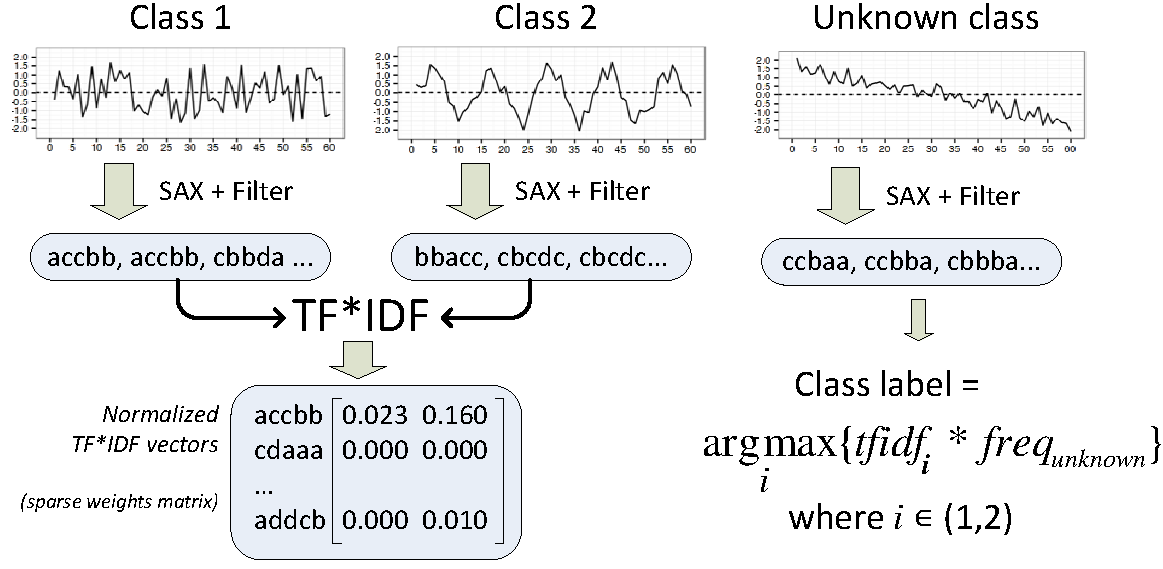
\includegraphics[width=90mm]{figures/overview.eps}
   \caption{
   An overview of SAX-VSM algorithm: 
   at first, labeled time series are converted into bags of words using SAX; 
   secondly, \textit{tf$\ast$idf} statistics is computed resulting in 
   a single weight vector per training class. For classification, an unlabeled 
   time series is converted into a term frequency vector and assigned a 
   label of a weight vector which yields a maximal cosine similarity value.
   This is \textit{ltc.nnn} weighting schema in SMART notation \cite{logtf}.}
   \label{fig:overview}
\end{figure}

\subsection{Training phase}
The training starts by transforming of all labeled time series into SAX representation
configured by four parameters: 
the sliding window length (\textit{W}), 
the number of PAA intervals per window (\textit{P}), 
the SAX alphabet size (\textit{A}), 
and by the numerosity reduction strategy (\textit{S}).
Each of the subsequences, extracted with overlapping sliding window, 
is normalized (Sec. \ref{section-sax}) before being processed with PAA. 
If, however, the standard deviation value falls below a fixed threshold, the 
normalization procedure is not applied in order to avoid a possible 
over-amplification of a background noise. 

By applying this procedure to all time series from $N$ training classes, 
algorithm builds a corpus of $N$ bags, to which, in turn, 
it applies \textit{tf$\ast$idf} ranking. 
These steps result in $N$ real-valued weight vectors of equal length 
representing $N$ training classes. 

Because of the need to scan the whole training set, training of SAX-VSM 
classifier is relatively computationally expensive ($O(nm)$). 
However, there is no need to maintain an index of training time series, 
or to keep any of them in the memory at the runtime: 
the algorithm simply iterates over all training time series incrementally building 
a single bag of SAX words for each of training classes. 
Once built and processed with \textit{tf$\ast$idf}, corpus is discarded - 
only a resulting set of $N$ real-valued weight vectors is retained for classification. 

\subsection{Classification}
In order to classify an unlabeled time-series, SAX-VSM transforms it into a
terms frequency vector using the same overlapping sliding window technique 
and SAX parameters that were used for training. 
Then, it computes cosine similarity values between this terms frequency vector 
and $N$ \textit{tf$\ast$idf} weight vectors representing the training classes. 
The unlabeled time series is assigned to the class whose vector yields the
maximal cosine similarity value.

\subsection{Sliding window size and SAX parameters selection} \label{section-direct}
As shown, SAX-VSM requires four parameters to be specified upfront. 
In order to optimize their selection using only a training data we adopt a common 
cross-validation technique and DIRECT optimization scheme \cite{direct-original}.
%However, DIRECT optimization scheme is designed to search for global minima of a real 
%valued function over a bound-constrained domain. In order to overcome this limitation, we 
%employ the rounding of reported solution values to the nearest integer.
Since DIRECT is designed to search for global minima of a real valued function 
over a bound constrained domain, we use the rounding of a reported solution values 
to the nearest integer.

DIRECT iteratively performs two procedures - partitioning the search domain and identifying 
potentially optimal hyper-rectangles.
%(i.e., having potential to contain good solutions). 
In our case, it begins by scaling the search domain to a 4-dimensional unit hypercube 
which is considered as potentially optimal. 
The error function is then evaluated at the center of this hypercube. Next, other points are 
created at one-third of the distance from the center in all coordinate directions. 
The hypercube is then divided into smaller rectangles that are identified by their center point 
and their error function value. This procedure continues interactively until error function
converges.
For brevity, we omit the detailed explanation of the algorithm, and refer the 
interested reader to \cite{direct} for additional details. Figure \ref{fig:direct-sampling} 
illustrates the application of DIRECT to \textit{SyntheticControl} data set problem, 
in this case, algorithm converged after sampling just 130 out of 13860 points.
% a 106X speedup

\begin{figure}[t]
   %\myfigureshrinker
   \centering
   \includegraphics[width=90mm]{figures/figure_direct.eps}
   \caption{Parameters optimization with DIRECT for \textit{SyntheticControl} data. 
   Left panel shows all points sampled by DIRECT in the space $PAA*Window*Alphabet$ where
   red points correspond to high error values in cross-validation experiments, 
   while green points indicate low error values. 
   Note the green points concentration at $W$=42. 
   Middle panel shows an error-rate heat map when the sliding window size is fixed to 42; 
   this plot was obtained by a complete scan of all 432 points of the slice. 
   Right panel shows the optimized by DIRECT sampling. The optimal solution 
   ($W$=42,$P$=8,$A$=4) was found by sampling of 43 points.}
   \label{fig:direct-sampling}
\end{figure}

\section{Results} \label{results}
We have proposed a novel algorithm for time series classification based on SAX
approximation of time series and Vector Space Model called SAX-VSM. 
Here, we present a range of experiments assessing its performance and show its 
ability to provide an insight into classification results.

\subsection{Analysis of the classification accuracy}
We evaluated our approach on 45 data sets whose majority was taken from benchmark 
data disseminated through UCR repository \cite{ucr}. While all the detail are available at 
project's homepage \cite{jmotif}, Table \ref{perf_table} compares the classification accuracy 
of SAX-VSM with previously published values of four competing classifiers: 
two state-of-the-art 1NN classifiers based on Euclidean distance and DTW, 
the classifier based on the recently proposed Fast-Shapelets technique \cite{fast-shapelets}, 
and the classifier based on BOP \cite{bag_patterns}.
We selected these particular techniques in order to position SAX-VSM in terms of 
classification accuracy and interpretability. 

In our evaluation, we followed a train/test data split as provided by UCR. 
Train data were used in cross-validation experiments for optimization of SAX parameters 
and numerosity reduction strategy using DIRECT. 
Once selected, optimal parameters was used to assess SAX-VSM classification accuracy 
which is reported in the last column of Table \ref{perf_table}.

\begin{footnotesize}
\begin{table}[t]
%\myfigureshrinkerless
\vspace{-0.3cm}
\caption{\bf Classifiers error rates comparison.}
 \label{perf_table}
\centering
\begin{tabularx}{\linewidth}{@{} l *6X @{}}
\hline
Data set & Nb. of classes & 1NN-Euclidean & 1NN-DTW & Fast Shapelets &  \mbox{Bag Of} \mbox{Patterns}
& SAX-VSM\\
\hline
Adiac        &37  & 0.389   & 0.391  & 0.514  & 0.432  & \textbf{0.381}\\
Beef         &5   & 0.467   & 0.467  & 0.447  & 0.433  & \textbf{0.033}\\
CBF         & 3  & 0.148    & 0.003  & 0.053    & 0.013 & \textbf{0.002} \\
Coffee       &2    & 0.250   & 0.180  & 0.067     & 0.036     & \textbf{0.0} \\
ECG200     &2   & \textbf{0.120}  & 0.230  & 0.227     & 0.140   & 0.140 \\
FaceAll      &14  & 0.286   & \textbf{0.192}  & 0.402     & 0.219   & 0.207\\
FaceFour    &4   & 0.216   & 0.170  & 0.089     & 0.011   & \textbf{0.0} \\
Fish         &7   & 0.217   & 0.167  & 0.197    & 0.074   & \textbf{0.017} \\
Gun-Point    &2   & 0.087   & 0.093  & 0.060     & 0.027     & \textbf{0.007} \\
Lightning2    &2   & 0.246   & \textbf{0.131}  & 0.295  & 0.164  & 0.196 \\
Lightning7    &7   & 0.425   & \textbf{0.274}  & 0.403  & 0.466  & 0.301 \\
Olive Oil     &4   & 0.133   & 0.133  & 0.213     & 0.133  & \textbf{0.100}\\
OSU Leaf    &6   & 0.483   & 0.409  & 0.359     & 0.236  & \textbf{0.107} \\
Syn.Control  &6   & 0.120   & \textbf{0.007}  & 0.081     & 0.037  & 0.010 \\
Swed.Leaf   &15  & 0.213   & 0.210 & 0.270 & \textbf{0.198} & 0.251 \\
Trace       &4   & 0.240   & \textbf{0.0}    & 0.002  & \textbf{0.0} & \textbf{0.0} \\
Two patterns &4   & 0.090   & \textbf{0.0}    & 0.113   & 0.129      & 0.004 \\
Wafer        &2    & 0.005   & 0.020     & 0.004  & 0.003 & \textbf{0.0006} \\
Yoga        &2    & 0.170   & \textbf{0.164}  & 0.249 & 0.170 & \textbf{0.164} \\
\hline
\vspace{0.1cm}
\end{tabularx}
\end{table}
\end{footnotesize}

\subsection{Scalability analysis} \label{scalability}
For synthetic data sets, it is possible to create as many instances as one needs for
experimentation.
We used CBF \cite{cbf} in order to investigate and compare the performance of 
SAX-VSM and 1NN Euclidean classifier on increasingly large data sets.

In one series of experiments, we varied a training size from 10 to 1000, while 
the test data set size remained fixed to 10'000 instances. 
For small training data sets, SAX-VSM was found to be significantly more accurate than 
1NN Euclidean classifier, but by the time we had more than 500 time series in a training set, 
there was no significant difference in accuracy (Fig. \ref{fig:precision-runtime}, left). 
As per the running time cost, due to the comprehensive training, SAX-VSM was found to 
be more expensive than 1NN Euclidean classifier on small training sets, 
but outperformed 1NN on large training sets. SAX-VSM allows to perform training offline and 
load weight vectors ``on demand'' - in this scenario, it performs classification significantly
faster than 1NN Euclidean classifier (Fig. \ref{fig:precision-runtime}, right).

In another series of experiments we investigated the scalability of our algorithm with
unrealistic training set sizes - up to 1'000'000 of instances of each of CBF classes.
As expected, with the grows of a training set size, the growth curve of a total number of 
distinct SAX words for each class' dictionary reflected significant dictionary saturation
peaking at 67'324 of distinct words (less than 10\% of all possible words of length 7
from 7 letters alphabet).
This result reflects SAX-VSM ability to learn from large datasets efficiently: 
while SAX smoothing limits the generation of new words corresponding to 
relatively similar sub-sequences, the \textbf{\textit{idf}} (Eq. \ref{formula:idf})
efficiently eliminates words that are loosing their discriminative power, 
i.e. those which appear in all classes.

\begin{figure}[t]
   %\myfigureshrinkerless
   \centering
   
\includegraphics[width=84mm]{figures/precision-runtime_new.ps}
   \caption{Comparison of classification precision and run time of SAX-VSM and 1NN 
   Euclidean classifier on CBF data. 
   Left: SAX-VSM performs significantly better with limited amount of training samples. 
   Center: while SAX-VSM is faster in time series classification, its performance 
   is comparable to 1NN Euclidean when training time is accounted for.
   Right: SAX-VSM increasingly outperforms 1NN Euclidean with noise level growth 
   (the random noise level varies up to 100\% of CBF signal value)
   }
   \label{fig:precision-runtime}
   \vspace{-0.1cm}
\end{figure}

%dictionary of the
%with While it grows rapidly at the beginning, once
%the dictionary is saturated, growth tend to slow down (left panel of Figure \ref{fig:corrupted}). 
%Nevertheless, by adjusting alphabet and PAA sizes it is possible to keep the number of terms
%significantly large. 
%\begin{figure}[t]
   %\myfigureshrinker
   %\centering
   %\includegraphics[width=84mm]{figures/Bubbles.eps}
   %\caption{Left panel: illustration of dictionaries size evolution for CBF with
   %increasingly large training set size. 
   %Right panel: distribution of SAX terms in CBF corpus for training set of 
   %one million series of each class.}
   %\label{fig:venn}
%\end{figure}

\subsection{Robustness to noise}
Since the weight of each of the overlapping SAX words is contributing only a small 
fraction to a final similarity value, prompted an idea that 
SAX-VSM classifier might be robust to the noise and to the partial loss of a signal in
test time series. Intuitively, in this case the cosine similarity between high dimensional 
weight vectors might not degrade significantly enough to cause a misclassification.

%\begin{figure}[t]
  %\myfigureshrinkerless
%  \centering
%  \includegraphics[width=84mm]{figures/corrupted.eps}
%  \caption{Classification performance with added noise
%  (left panel; the random noise level varies up to 100\% of the signal value,
%  and with a signal loss (right panel). \textit{SAX-VSM Opt} curves correspond to 
%  results obtained with ``optimized'' for each case SAX parameters 
%  (we re-trained a classifier).}
%  \label{fig:corrupted}
% \end{figure}

We investigated this hypothesis using CBF data. By fixing a training set size to 250 
time series, we varied the standard deviation of Gaussian noise in CBF model.
%(whose default value is about 17\% of a signal level). We found, that SAX-VSM 
%increasingly outperformed 1NN
SAX-VSM outperformed 1NN Euclidean classifier with the growth of a noise level 
confirming our hypothesis (Fig.\ref{fig:precision-runtime}). 
Further improvement of SAX-VSM performance was achieved by fine tuning of smoothing 
through a gradual increase of the SAX sliding window size proportionally to the growth of 
the noise level (\textit{SAX-VSM Opt} curve, Fig.\ref{fig:precision-runtime}). 

%In other experiments, we randomly replaced up to 50\% of a span of an 
%unlabeled time series with a random noise. Again, SAX-VSM performed consistently better 
%than 1NN Euclidean classifier regardless of a training set size, which we varied from 
%five to one thousand. The \textit{SAX-VSM Opt} curve at Fig.\ref{fig:corrupted} (Right) depicts
%the case with 50 series when the sliding window size was decreased inversely proportionally 
%to the growth of a signal loss.


\begin{figure}[b]
   %\myfigureshrinker
   \centering
   \vspace{0.3cm}
   \includegraphics[width=87mm]{figures/CBF-HEAT.eps}
   \caption{An example of the heatmap-like visualization of subsequence ``importance''
   to a class identification. 
   Here, for three CBF time series from a training set, a color value 
   of each point was obtained by combining tf$\ast$idf weights of all patterns 
   which cover the point.
   If a pattern was found in a SAX-VSM-built dictionary corresponding to the 
   time-series class, we added its weight, if, however, a pattern was found in 
   another dictionary - we subtracted its weight. Highlighted by the visualization 
   features corresponding to a sudden rise, plateau, and a sudden drop in Cylinder;
   increasing trend in Bell;
   and to a sudden rise followed by a gradual drop in Funnel, align exactly with the
   design of these classes \cite{cbf}.}
   \label{fig:heat}
   \vspace{-0.5cm}
\end{figure}

\subsection{Interpretable classification}
While the classification performance results show that SAX-VSM classifier has 
a very good potential, its major strength is in the level of allowed 
interpretability of classification results. 

Previously, it was shown by the authors, that the shapelet-based decision tree provides 
interpretable classification and offers an insight into the data specific features \cite{shapelet}. 
Later, it was shown that the discovery of multiple shapelets provides even 
better resolution and intuition into the interpretability of classification \cite{bagnal}. 
However, as the authors noted, a time cost of multiple shapelets discovery
in many class problems could be very significant. 
Contrary, SAX-VSM extracts and weights all patterns at once without
any added cost. Thus, it could be the only choice for interpretable classification 
in many class problems. 
Here, we show a few examples in which we exploit the subsequence ranking 
data provided by our technique.

\subsubsection{Heatmap-like visualization}
Since SAX-VSM outputs tf$\ast$idf weight vectors of all subsequences extracted from a
class, it is possible to find out a weight of any arbitrary selected subsequence.
This feature enables a novel visualization technique that can be used to gain an immediate
insight into the layout of ``important'' class-characterizing subsequences as shown at Figure
\ref{fig:heat}.

\begin{figure}[]
   %\myfigureshrinker
   \centering
   \includegraphics[width=87mm]{figures/gun-point.eps}
   \caption{Best characteristic subsequences (right panels, bold lines) discovered by SAX-VSM in
   \textit{Gun/Point} data set. 
   Left panel shows actor's stills and time series annotations made by an expert, 
   right panels show locations of characteristic subsequences.
   Note, that while the upward arm motion found to be more ``important'' in \textit{Gun} 
   class (gun retrieval and aiming), the downward arm motion better characterizes 
   \textit{Point} class (an ``overshoot'' phenomena in propless arm return). 
   This result aligns with previous work \cite{shapelet} and \cite{bagnal}.
   (Stills and annotation used with a permission from E. Keogh) }
   \label{fig:shapelet-like-patterns}
\end{figure}

\subsubsection{Gun Point data set}
Following previous shapelet-based work \cite{shapelet} \cite{bagnal}, 
we used a well-studied \textit{GunPoint} data set \cite{gun} to explore the 
interpretability of classification results. The class \textit{Gun} of this dataset 
corresponds to the actors' hands motion when drawing a replicate gun from 
a hip-mounted holster, pointing it at a target for a second, and returning the 
gun to the holster; class \textit{Point} correspond to the actors hands motion 
when pretending of drawing a gun - the actors point their index fingers to 
a target for about a second, and then return their hands to their sides. 

Similarly to previously reported results, SAX-VSM was able to capture all 
distinguishing features as shown at the Figure \ref{fig:shapelet-like-patterns}. 
The top weighted by SAX-VSM patterns in \textit{Gun} class corresponds 
to fine movements required to lift and aim the prop. 
The top weighted SAX pattern in \textit{Point} class corresponds to the 
``overshoot'' phenomena causing the dip in the time series \cite{gun}, 
while the second to best pattern captures the lack of movements
required for lifting a hand above a holster and reaching down for the prop. 

\subsubsection{OSU Leaf data set}
The \textit{OSULeaf} data set consist of curves obtained by color image segmentation 
and boundary extraction from digitized leaf images of six classes \cite{osuleaf}.
The authors were able to solve the problem of leaf boundary curves classification 
by use of DTW, achieving 61\% of classification accuracy. 
However, DTW provided a very little information about why it succeeded of failed. 
In contrast, SAX-VSM application yielded a set of class-specific characteristic 
patterns for each of six leaves classes which closely match known techniques 
of leaves classification based on leaf shape and margin \cite{dirr}. 
Highlighted by SAX-VSM features include the slightly lobed shape and acute tips of
Acer Circinatum leaves, serrated blade of Acer Glabrum leaves, the acuminate tip and characteristic
serration of in Acer Macrophyllum leaves, pinnately compound leaves arrangement of Acer Negundo, the
incised leaf margin of Quercus Kelloggii, and a lobed leaf structure of Quercus Garryana 
(Figure \ref{fig:shapelet-acer-patterns}).

\begin{figure}[t]
   %\myfigureshrinker
   \centering
   \vspace{-0.2cm}
   \includegraphics[width=87mm]{figures/AcerCircunatum.eps}
   \caption{Example of best characteristic subsequences (top panels, bold lines) discovered 
   by SAX-VSM in \textit{OSULeaf data set}.
    These patterns align with known in botany discrimination techniques based on lobe shapes, 
    serrations, and leaf tip types \cite{dirr}.}
   \label{fig:shapelet-acer-patterns}
   \vspace{-0.2cm}
\end{figure}

\subsubsection{Coffee data set}
Similarly to the original work based on PCA \cite{coffee}, in both classes Coffee spectrograms, 
SAX-VSM highlighted intervals corresponding to Chlorogenic acid (best) and Caffeine 
(second to best) - the two chemical compounds that are known to be responsible for the flavor 
differences in Arabica and Robusta coffees.

% \section{Clustering}
% Clustering is a common tool used for data partitioning, visualization, exploration, and serves as
% an important subroutine in many data mining algorithms. Typically, clustering algorithms
% are built upon a distance function, and the overall performance of an algorithm is highly
% dependent on a performance of the chosen function. Thus, an experimental evaluation of the 
% proposed technique in clustering provides an additional perspective on its performance and
% applicability beyond the classification.
% 
% \subsection{Hierarchical clustering}
% Probably, one of the most used clustering algorithms is hierarchical clustering which requires no
% parameters to be specified \cite{hcs}. It computes pairwise distances between all objects and 
% produces a nested hierarchy of clusters offering a great data visualization power. 
% 
% Previously, it was shown that the bag-of-patterns time series representation and Euclidean distance
% provide a superior clustering performance\cite{bag_patterns}. 
% For comparison, we performed similar experiments which differ in time series representation and
% distance metric - we relied on \textit{tf$\ast$idf} weight vectors and cosine similarity. 
% Affirming the previous work, we found, that the combination of SAX and Vector space model
% outperforms classical shape-based distance metrics. 
% For example, figure \ref{fig:hc} depicts the result of hierarchical clustering of a subset of
% \textit{SyntheticControl} data. 
% As one can see, SAX-VSM is superior in clustering performance to Euclidean and DTW distance 
% metrics in this particular setup - it produced a hierarchy which properly partitions the
% data set into three branches.
% 
% \subsection{k-Means clustering}
% Another popular choice for data partitioning is k-Means clustering algorithm \cite{kmeans}.
% The basic intuition behind this algorithm is that through the iterative reassignment of objects 
% into different clusters the intra-cluster distance is minimized. As was shown, k-Means 
% algorithm scales much better than hierarchical partitioning techniques \cite{kscale}.
% Fortunately, this clustering technique is well studied in IR field. Previously, in \cite{zhao}, the
% authors extensively examined seven different criterion functions for partitional document
% clustering and found, that \textit{k}-prototypes partitioning with cosine dissimilarity delivers an
% excellent performance. 
% 
% Following this work, we implemented a similar to \cite{modha} \textit{spherical k-means algorithm}
% and found, that algorithm converges quickly and delivers a satisfactory partitioning on short
% synthetic data sets. Further, we evaluated our technique on the long time series from PhysioNet 
% archive \cite{physionet}. 
% We extracted two hundred fifty series corresponding to five vital signals: two ECG leads 
% (aVR and II), and RESP, PLETH, and CO2 waves, trimming them to 2'048 points. Similarly to
% \cite{bag_patterns}, we run a reference k-Means algorithm implementation based on Euclidean
% distance, which achieved the maximum clustering quality of 0.39, when measured as proposed in
% \cite{kmetrics} on the best clustering (the one with the smallest objective function in 10 runs). 
% SAX-VSM spherical k-Means implementation outperformed the reference technique yielding 
% clusters  with the quality of 0.67 (on 10 runs with SAX parameters set to 
% $W$=33, $P$=8, $A$=6).
% 
% %Note also, that previously, we applied our implementation to recurrent behaviors (motifs) 
% %discovery in software development telemetry streams\cite{android}. 
% %These behavioral time series were extracted from software change repositories and are 
% %structurally similar to \textit{ElectricDevices} data set. 
% %We used our \textit{tf$\ast$idf} weight vectors time series representation and spherical 
% %k-Means implementation in order to discover specific temporal features corresponding 
% %to the software release cycle. 
% %Specifically, we optimized SAX parameters in order to obtain a proper partitioning of known 
% %development behaviors before and after the software release. 
% %In turn, the centroids of these clusters represented by \textit{tf$\ast$idf} weight vectors 
% %were used to classify unlabeled  temporal intervals. 
% %This technique allowed us to successfully classify pre- and post-release
% %behaviors with accuracy above 80\%.
% 
% \begin{figure}[t]
%    %\myfigureshrinker
%    \centering
%    \includegraphics[width=87mm]{figures/clustering.eps}
%    \caption{An comparison of hierarchical clustering application to a subset of three
%    \textit{SyntheticControl} classes: \textit{Normal, Decreasing trend}, and \textit{Upward shift}. 
%    Euclidean distance, Dynamic time warping, SAX-VSM and Complete linkage were used to 
%    generate these plots. Only SAX-VSM was able to partition series properly.                       
%    }
%    \label{fig:hc}
% \end{figure}

\section{Conclusion and Future Work} \label{conclusion}
In this paper, we have proposed a novel interpretable technique for time series classification
based on characteristic patterns discovery. We have shown, that our approach is competitive with, 
or superior to, other techniques on a set of classic data mining problems. In addition, 
we described several advantages of SAX-VSM over existing structure-based similarity measures,
emphasizing its capacity to discover and rank short subsequences by their class characterization
power.

\begin{figure}[t]
   %\myfigureshrinker
   \centering
   \vspace{-0.2cm}
   \includegraphics[width=84mm]{figures/coffee_patterns.ps}
   \caption{
   Best characteristic subsequences (left panels, bold lines) discovered by SAX-VSM in
   {Coffee data set}. Right panels show zoom-in view on these subsequences in Arabica
   and Robusta spectrograms.
   These discriminative subsequences correspond to chlorogenic acid (best subsequence) 
   and to caffeine (second to best) regions of spectra. This result aligns with
   the original work based on PCA \cite{coffee} exactly.
   %Best characteristic subsequences discovered by SAX-VSM in \textit{Coffee data set}.
   %The best subsequences in both classes correspond to chlorogenic acid, while
   %second to best subsequences - to caffeine. This result aligns with previous 
   %exploratory research based on PCA \cite{coffee}.
   }
   \label{fig:coffee}
   \vspace{-0.2cm}
\end{figure}

%First of all, by combining \textit{all} SAX words extracted from \textit{all} time series of a 
%class into a \textit{single bag} of words, SAX-VSM manages not only to capture presented intraclass variability, 
%but to efficiently ``generalize'' it through smoothing with PAA and SAX.  

%Secondly, by partially discarding the original ordering of time series subsequences and
%through subsequence normalization, SAX-VSM is capable to capture, and to recognize 
%characteristic subsequences in distorted by rotation or shift time series, as well,
%as to recover a signal from partially corrupted or altered by noise data. 

%Thirdly, the \textit{tf$\ast$idf} statistics naturally ``highlights'' terms unique to a
%class by assigning them higher weights, while terms observed in multiple classes are 
%assigned weights inversely proportional to their interclass presence frequency. 
%This weighting scheme improves the selectivity of classification by lowering a 
%contribution of ``confusive'' multi-class terms while increasing that of
%class' ``defining'' terms to a final similarity value.   


%When combined, these features make SAX-VSM time series classification approach 
%unique. 
%Ultimately, algorithm classifies an unknown time series is classified by
%its similarity not to a given number of ``neighbors'' (as in kNN or BOP classifiers), 
%or to a pre-defined number of characteristic features (as in shapelets-based classifiers), 
%but by its subsequences similarity to all ranked by characteristic power discriminative 
%subsequences found in a whole training class.
%As we shall show, this contributes to the excellent classification performance in two 
%usually difficult scenarios: when only a small training set is available, 
%and when time series have a very low intraclass similarity at the full length, 
%but embed characteristic to the class subsequences. 

The current limitations of our SAX-VSM implementation suggest a number of future work directions. 
First of all, inspired by the recently reported superior performance of multi-shapelets based classifiers
\cite{bagnal}, we prioritize extension of our algorithm in order to accept SAX words of variable length.
Secondly, we are working on alternative parameter optimization scheme in order to reduce classifier 
training time. Finally, we are evaluating an extension to multidimensional time series.

% An example of a floating figure using the graphicx package.
% Note that \label must occur AFTER (or within) \caption.
% For figures, \caption should occur after the \includegraphics.
% Note that IEEEtran v1.7 and later has special internal code that
% is designed to preserve the operation of \label within \caption
% even when the captionsoff option is in effect. However, because
% of issues like this, it may be the safest practice to put all your
% \label just after \caption rather than within \caption{}.
%
% Reminder: the "draftcls" or "draftclsnofoot", not "draft", class
% option should be used if it is desired that the figures are to be
% displayed while in draft mode.
%
%\begin{figure}[!t]
%\centering
%\includegraphics[width=2.5in]{myfigure}
% where an .eps filename suffix will be assumed under latex, 
% and a .pdf suffix will be assumed for pdflatex; or what has been declared
% via \DeclareGraphicsExtensions.
%\caption{Simulation Results}
%\label{fig_sim}
%\end{figure}

% Note that IEEE typically puts floats only at the top, even when this
% results in a large percentage of a column being occupied by floats.


% An example of a double column floating figure using two subfigures.
% (The subfig.sty package must be loaded for this to work.)
% The subfigure \label commands are set within each subfloat command, the
% \label for the overall figure must come after \caption.
% \hfil must be used as a separator to get equal spacing.
% The subfigure.sty package works much the same way, except \subfigure is
% used instead of \subfloat.
%
%\begin{figure*}[!t]
%\centerline{\subfloat[Case I]\includegraphics[width=2.5in]{subfigcase1}%
%\label{fig_first_case}}
%\hfil
%\subfloat[Case II]{\includegraphics[width=2.5in]{subfigcase2}%
%\label{fig_second_case}}}
%\caption{Simulation results}
%\label{fig_sim}
%\end{figure*}
%
% Note that often IEEE papers with subfigures do not employ subfigure
% captions (using the optional argument to \subfloat), but instead will
% reference/describe all of them (a), (b), etc., within the main caption.


% An example of a floating table. Note that, for IEEE style tables, the 
% \caption command should come BEFORE the table. Table text will default to
% \footnotesize as IEEE normally uses this smaller font for tables.
% The \label must come after \caption as always.
%
%\begin{table}[!t]
%% increase table row spacing, adjust to taste
%\renewcommand{\arraystretch}{1.3}
% if using array.sty, it might be a good idea to tweak the value of
% \extrarowheight as needed to properly center the text within the cells
%\caption{An Example of a Table}
%\label{table_example}
%\centering
%% Some packages, such as MDW tools, offer better commands for making tables
%% than the plain LaTeX2e tabular which is used here.
%\begin{tabular}{|c||c|}
%\hline
%One & Two\\
%\hline
%Three & Four\\
%\hline
%\end{tabular}
%\end{table}


% Note that IEEE does not put floats in the very first column - or typically
% anywhere on the first page for that matter. Also, in-text middle ("here")
% positioning is not used. Most IEEE journals/conferences use top floats
% exclusively. Note that, LaTeX2e, unlike IEEE journals/conferences, places
% footnotes above bottom floats. This can be corrected via the \fnbelowfloat
% command of the stfloats package.



%\section{Conclusion}
%The conclusion goes here.




% conference papers do not normally have an appendix


% use section* for acknowledgement
%\section*{Acknowledgment}


%The authors would like to thank...





% trigger a \newpage just before the given reference
% number - used to balance the columns on the last page
% adjust value as needed - may need to be readjusted if
% the document is modified later
%\IEEEtriggeratref{8}
% The "triggered" command can be changed if desired:
%\IEEEtriggercmd{\enlargethispage{-5in}}

% references section

% can use a bibliography generated by BibTeX as a .bbl file
% BibTeX documentation can be easily obtained at:
% http://www.ctan.org/tex-archive/biblio/bibtex/contrib/doc/
% The IEEEtran BibTeX style support page is at:
% http://www.michaelshell.org/tex/ieeetran/bibtex/
\bibliographystyle{IEEEtran}
% argument is your BibTeX string definitions and bibliography database(s)
%\bibliography{IEEEabrv,../bib/paper}
%
% <OR> manually copy in the resultant .bbl file
% set second argument of \begin to the number of references
% (used to reserve space for the reference number labels box)
\begin{thebibliography}{5}
%1
\bibitem {review}
Wang, X., Mueen, A., Ding, H., Trajcevski, G., Scheuermann, P., Keogh, E.:
Experimental comparison of representation methods and distance measures for time series data.
DMKD, 26, 2, 275--309 (2013)

%2
%\bibitem {survey}
%Xing, Z., Pei, J., Keogh, E.:
%A brief survey on sequence classification. 
%SIGKDD Explor. Newsl. 12, 1, 40-48, (2010)

%3
\bibitem {benchmark}
Keogh, E., Kasetty, S.:
On the need for time series data mining benchmarks: a survey and empirical demonstration.
DMKD, 7, 4, 349--371 (2003)

%2
\bibitem {comparison}
Ding, H., Trajcevski, G., Scheuermann, P., Wang, X., Keogh, E.:
Querying and mining of time series data: experimental comparison of representations and distance
measures. 
In Proc. VLDB, 1542--1552 (2008)

%3
\bibitem {1NN}
Xi, X., Keogh, E., Shelton, C., Wei, L., Ratanamahatana, C.:
Fast time series classification using numerosity reduction. 
In Proc. ICML, 1033--1040 (2006)

%3
\bibitem {DTW}
Sakoe, H. Chiba, S.:
Dynamic programming algorithm optimization for spoken word recognition.
IEEE Trans. on Acoustics, Speech and Signal Processing, 1, 43--49 (1978)

	
%\bibitem {spade}
%Chen, Y., Chen, K., Nascimento, M.:
%Effective and Efficient Shape-Based Pattern Detection over Streaming Time Series. 
%IEEE TKDE, 265--278 (2012)

%4
\bibitem {DFT}
Agrawal, R., Faloutsos, C., Swami, A.:
Efficient Similarity Search In Sequence Databases.
In Proc. FODO, 69--84 (1993)

%5
\bibitem {bag_patterns}
Lin, J., Khade, R., Li, Y.:
Rotation-invariant similarity in time series using bag-of-patterns representation. 
J. Intell. Inf. Syst. 39, 2, 287--315 (2012)

%6

%7
%\bibitem {indexing}
%Keogh, E.:
%Exact indexing of dynamic time warping. 
%In Proc. VLDB, 406--417 (2002)

%8
\bibitem {shapelet}
Ye, L., Keogh, E.:
Time series shapelets: a novel technique that allows accurate, interpretable and fast
classification. 
DMKD, 22, 149--182 (2011)

%9
%\bibitem {logical}
%Mueen, A., Keogh, E., Young, N.:
%Logical-shapelets: an expressive primitive for time series classification.
%In Proc. 17th ACM SIGKDD, 1154--1162 (2011)

%10
\bibitem {bagnal}
Lines, J., Davis, L., Hills, J., Bagnall, A.:
A shapelet transform for time series classification. 
In Proc. 18th ACM SIGKDD, 289--297 (2012)

%11

%12
\bibitem {classifiers}
Salzberg, S.:
On comparing classifiers: Pitfalls to avoid and a recommended approach. 
DMKD, 1, 317--328 (1997)

%13
\bibitem {sax}
Lin, J., Keogh, E., Wei, L., Lonardi, S.:
Experiencing SAX: a novel symbolic representation of time series.
DMKD, 107--144 (2007)

%14
\bibitem {salton}
Salton, G., Wong, A., Yang., C.:
A vector space model for automatic indexing. 
Commun. ACM 18, 11, 613--620 (1975)

%15
\bibitem {direct}
Bj\"{o}rkman, M., Holmstr\"{o}m, K.:
Global Optimization Using the DIRECT Algorithm in Matlab.
Adv. Modeling and Optimization, 1, 17-37 (1999)

%16
\bibitem {hot_sax}
Keogh, E., Lin, J., Fu, A.:
HOT SAX: Efficiently Finding the Most Unusual Time Series Subsequence. 
In Proc. ICDM. 226--233 (2005)

%17
\bibitem {fast-shapelets}
Rakthanamanon, T., Keogh, E.:
Fast-Shapelets: A Scalable Algorithm for Discovering Time Series Shapelets.
In Proc. SDM (2013)

%18
\bibitem {goldin_kanellakis}
Goldin D., Kanellakis, P.:
On Similarity Queries for Time-Series Data: Constraint Specification and Implementation. 
In Proc CP. 137--153 (1995)

%not used
\bibitem {paa}
Keogh, E., Pazzani, M.:
A Simple Dimensionality Reduction Technique for Fast Similarity Search in Large Time Series
Databases. In Proc. PADKK, 122--133 (2000)

%19
%\bibitem {larsen_marx}
%Larsen, R., Marx, M.:
%An Introduction to Mathematical Statistics and Its Applications, (3rd Ed.),
%Prentice Hall (2000)

%20
%\bibitem {motifs}
%Chiu, B., Keogh, E., Lonardi, S.:
%Probabilistic discovery of time series motifs. 
%In Proc. 9th ACM SIGKDD (2003)

\bibitem {logtf}
Manning, C., Raghavan, P., Sch\"utze, H.: 
Introduction to Information Retrieval, Cambridge University Press (2008)

%21
\bibitem {streaming_sax}
Lin, J., Keogh, E., Lonardi, S., Chiu, B.:
A symbolic representation of time series, with implications for streaming algorithms. 
In Proc. 8th DMKD. 2--11 (2003)

%22
\bibitem {hamming}
Hamming, R.:
Error detecting and error correcting codes. 
Bell System Technical Journal 29, pp. 147--160 (1950)

%23
\bibitem {jmotif}
Paper authors. Supporting webpage:
%Paper Authors:
%Accompanying information for this paper. 
\url{https://code.google.com/p/jmotif/}

%24
\bibitem {direct-original}
Jones, D., Perttunen, C., Stuckman, B.:
Lipschitzian Optimization without Lipschitz Constant.
J. Optim. Theory Appl. 79, 1 (1993)

%25
\bibitem {ucr}
Keogh, E., Zhu, Q., Hu, B., Hao, Y.,  Xi, X., Wei, L., Ratanamahatana, C.:
The UCR Time Series Classification/Clustering Homepage:
\url{http://www.cs.ucr.edu/~eamonn/time_series_data/}

%26
%\bibitem {ford}
%WCCI, Ford classification challenge,
%\url{http://home.comcast.net/~nn_classification/}

%27
\bibitem {nfl}
Wolpert, D., Macready, W.:
No free lunch theorems for optimization.
IEEE Trans. on Evo. Comp. 1 no. 1, 67--82 (1997)

%28
\bibitem {cbf}
Saito, N:
Local feature extraction and its application using a library of bases. 
PhD thesis, Yale University (1994)

%38
%\bibitem {android}
%Senin, P.: 
%Recognizing recurrent development behaviors corresponding to Android OS release life-cycle.
%In Proc. SERP (2012)

%29
\bibitem {gun}
Ratanamahatana, C., Keogh, E.:
Making time-series classification more accurate using learned constraints. 
In SDM '04 (2004)

%30
\bibitem {osuleaf}
Gandhi, A.:
Content-Based Image Retrieval: Plant Species Identification. 
MS thesis, Oregon State University (2002)

%31
\bibitem {dirr}
Dirr, M.:
Manual of Woody Landscape Plants: Their Identification, Ornamental Characteristics,
Culture, Propogation and Uses.
Stipes Pub Llc, ed. 6 Revised (2009)

%32
\bibitem {coffee}
Briandet, R., Kemsley, E., Wilson, R.:
Discrimination of Arabica and Robusta in Instant Coffee by Fourier Transform Infrared Spectroscopy
and Chemometrics.
J. Agric. Food Chem, 44, 170--174 (1996)

%33
%\bibitem {hcs}
%Johnson, C.:
%Hierarchical clustering schemes.
%Psychometrika, 32(3), 241--254 (1967)

%34
%\bibitem {kmeans}
%MacQueen, J.:
%Some methods for classification and analysis of multivariate observations
%Proc. of 5th Berkeley Symp. On  Math. Stat. and Prob., 1, 281--296 (1967)

%35
%\bibitem {kscale}
%Bradley, P., Fayyad, U., Reina, C.:
%Scaling clustering algorithms to large databases. 
%In Proc. KDD, 9--15 (1998)

%\enlargethispage{0.5cm} 
%36
%\bibitem {zhao}
%Zhao, Y., Karypis, G.:
%Empirical and Theoretical Comparisons of Selected Criterion Functions for Document Clustering.
%Mach. Learn., 55, 311--331 (2004)

%37
%\bibitem {modha}
%Dhillon, I., Modha, D.:
%Concept Decompositions for Large Sparse Text Data Using Clustering.
%Mach. Learn., 42(1), 143--175 (2001)

%\bibitem {physionet}
%Goldberger, A., Amaral, L., Glass, L., et al.: PhysioBank, PhysioToolkit, and 
%PhysioNet: Circulation. Discovery 101(23), 1(3), 215--220 (1997) 

%\bibitem {kmetrics}
%Gavrilov, M., Anguelov, D., Indyk, P., Motwani, R.:
%Mining the stock market: which measure is best? 
%In Proc. 6th KDD. 487--496 (2000)
\end{thebibliography}


% that's all folks
\end{document}


